\documentclass[11pt,a4paper]{article}
\usepackage[margin=1in]{geometry}
\usepackage{amsmath}
\usepackage{amssymb}
\usepackage{titlesec}
\usepackage{enumitem}
\usepackage{xcolor}
\usepackage[most]{tcolorbox}
\usepackage{fancyhdr}
\usepackage{listings}
\usepackage{hyperref}
\usepackage{graphicx}
\usepackage{tikz}
\usetikzlibrary{shapes.geometric, arrows, positioning}

\newcommand{\wrongmark}{\times}
\usepackage[utf8]{inputenc}
\usepackage{newunicodechar} 
\newunicodechar{✓}{\checkmark}
\newunicodechar{✗}{\wrongmark}
\DeclareUnicodeCharacter{2502}{|}
\DeclareUnicodeCharacter{251C}{+}
\DeclareUnicodeCharacter{2500}{-}
\DeclareUnicodeCharacter{2514}{+}

% Header and Footer
\pagestyle{fancy}
\fancyhf{}
\rhead{FastAPI Complete Guide}
\lhead{Patient Management System}
\cfoot{\thepage}

% Title formatting
\titleformat{\section}{\Large\bfseries\color{blue!70!black}}{\thesection}{1em}{}[\titlerule]
\titleformat{\subsection}{\large\bfseries\color{blue!50!black}}{\thesubsection}{1em}{}
\titleformat{\subsubsection}{\normalsize\bfseries\color{blue!40!black}}{\thesubsubsection}{1em}{}

% Code styling
\definecolor{codebg}{gray}{0.95}
\definecolor{codegreen}{rgb}{0,0.6,0}
\definecolor{codegray}{rgb}{0.5,0.5,0.5}
\definecolor{codepurple}{rgb}{0.58,0,0.82}

\lstdefinestyle{pythonstyle}{
    language=Python,
    backgroundcolor=\color{codebg},
    commentstyle=\color{codegreen},
    keywordstyle=\color{blue},
    numberstyle=\tiny\color{codegray},
    stringstyle=\color{codepurple},
    basicstyle=\ttfamily\small,
    breaklines=true,
    captionpos=b,
    keepspaces=true,
    numbers=left,
    numbersep=5pt,
    showspaces=false,
    showstringspaces=false,
    showtabs=false,
    tabsize=4,
    frame=single,
    xleftmargin=2em,
    framexleftmargin=1.5em
}

\lstdefinestyle{bashstyle}{
    language=bash,
    backgroundcolor=\color{codebg},
    basicstyle=\ttfamily\small,
    breaklines=true,
    frame=single,
    xleftmargin=2em,
    framexleftmargin=1.5em
}

\lstset{style=pythonstyle}

% Command box
\newtcolorbox{cmdbox}{
    colback=codebg,
    colframe=black!50,
    boxrule=0.5pt,
    left=2mm,
    right=2mm,
    top=1mm,
    bottom=1mm,
    breakable
}

% Example box
\newtcolorbox{examplebox}[1]{
    colback=green!5!white,
    colframe=green!75!black,
    title=#1,
    fonttitle=\bfseries,
    breakable,
    enhanced jigsaw
}

% Note box
\newtcolorbox{notebox}{
    colback=yellow!10!white,
    colframe=orange!75!black,
    title=Important Note,
    fonttitle=\bfseries,
    breakable,
    enhanced jigsaw
}

% Warning box
\newtcolorbox{warningbox}{
    colback=red!5!white,
    colframe=red!75!black,
    title=Warning,
    fonttitle=\bfseries,
    breakable,
    enhanced jigsaw
}

% Info box
\newtcolorbox{infobox}[1]{
    colback=blue!5!white,
    colframe=blue!75!black,
    title=#1,
    fonttitle=\bfseries,
    breakable,
    enhanced jigsaw
}

\begin{document}

% Title Page
\begin{titlepage}
    \centering
    \vspace*{2cm}
    {\Huge\bfseries FastAPI\\[0.5cm] Patient Management System\par}
    \vspace{1cm}
    {\Large Complete Backend Development Guide\par}
    \vspace{2cm}
    {\large A Comprehensive Guide to Building REST APIs,\\
    HTTP Methods, CRUD Operations, and FastAPI Project Development\par}
    \vspace{3cm}
    {\Large\bfseries Sujil S\par}
    \vspace{0.5cm}
    {\large\texttt{sujil9480@gmail.com}\par}
    \vfill
    {\large \today\par}
\end{titlepage}

\tableofcontents
\newpage

% ========================
% SECTION 1: PROJECT OVERVIEW
% ========================
\section{Project Overview}

\subsection{Introduction}

Welcome to the FastAPI Patient Management System project! This comprehensive guide will walk you through building a fully functional REST API from scratch. This project represents a real-world backend application that solves an actual problem faced by healthcare professionals.

\subsection{The Problem Statement}

\subsubsection{Current Situation}

When you visit a doctor's clinic, you've probably noticed a common practice:

\begin{itemize}[leftmargin=*]
    \item Doctors provide prescriptions on clinic letterhead
    \item They write remarks and medicine names by hand
    \item Patients are asked to bring these documents on next visit
    \item Over the years, you accumulate a file of paper prescriptions
    \item These papers can get misplaced or lost
    \item Both patient and doctor maintain physical copies
\end{itemize}

\begin{notebox}
\textbf{The Core Problem}: This entire system is offline and prone to data loss. There's no centralized, digital record keeping system. Papers can be lost, making it difficult to track medical history accurately.
\end{notebox}

\subsubsection{Our Solution}

We're building a startup that digitizes this entire process:

\begin{enumerate}[leftmargin=*]
    \item \textbf{Digital Platform}: Provide doctors with an app/system
    \item \textbf{Patient Profiles}: Doctors can maintain profiles for each patient
    \item \textbf{Centralized Storage}: All patient records stored in one place
    \item \textbf{Easy Access}: Quick retrieval of patient history
    \item \textbf{Data Management}: Create, view, update, and delete patient records
\end{enumerate}

\subsection{Patient Profile Structure}

A typical patient profile in our system contains:

\begin{center}
\begin{tabular}{|l|l|}
\hline
\textbf{Field} & \textbf{Description} \\
\hline
Name & Patient's full name \\
\hline
City & Location of patient \\
\hline
Age & Patient's age \\
\hline
Gender & Male/Female/Other \\
\hline
Height & Height in meters \\
\hline
Weight & Weight in kilograms \\
\hline
BMI & Body Mass Index (calculated) \\
\hline
\end{tabular}
\end{center}

\begin{notebox}
While a real-world medical system would have much more information (medical history, allergies, current medications, etc.), we're keeping it simple for this learning project. However, the same principles can be extended to include any amount of data.
\end{notebox}

\subsection{What We're Building}

\subsubsection{Our Task as Backend Engineers}

\begin{infobox}{Important Distinction}
We are NOT building the actual app (that's frontend work). We're building the \textbf{API} - the backend system that the app will communicate with.
\end{infobox}

\textbf{The API will provide approximately 5 endpoints}:

\begin{enumerate}[leftmargin=*]
    \item \textbf{Create Patient}: Add new patient records
    \item \textbf{View All Patients}: Retrieve all patient records
    \item \textbf{View Specific Patient}: Get details of one patient by ID
    \item \textbf{Update Patient}: Modify existing patient information
    \item \textbf{Delete Patient}: Remove patient from database
\end{enumerate}

\subsection{Data Storage Approach}

\subsubsection{Development vs Production}

\hspace{1.5em}\textbf{Ideal Approach}: Store data in a proper database (PostgreSQL, MongoDB, etc.)

\textbf{Our Approach}: For this learning project, we'll use a JSON file

\begin{notebox}
Using a JSON file instead of a database doesn't change the fundamental logic. The methods and operations remain the same. This approach helps us focus on API development without the complexity of database setup.
\end{notebox}

\subsection{API Functionality Overview}

\begin{center}
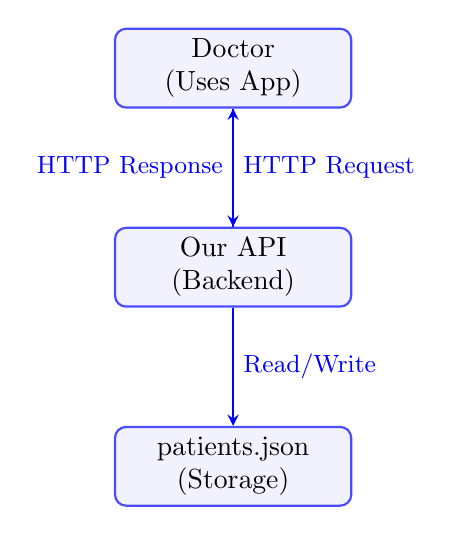
\begin{tikzpicture}[
    node distance=1.5cm,
    box/.style={rectangle, rounded corners, draw=blue!70, fill=blue!5, thick, minimum width=3cm, minimum height=1cm, align=center},
    arrow/.style={->, >=stealth, thick, blue}
]

% Main boxes
\node[box] (doctor) {Doctor\\(Uses App)};
\node[box, below=1.5cm of doctor] (api) {Our API\\(Backend)};
\node[box, below=1.5cm of api] (json) {patients.json\\(Storage)};

% Arrows with labels
\draw[arrow] (doctor) -- node[right, font=\small] {HTTP Request} (api);
\draw[arrow] (api) -- node[left, font=\small] {HTTP Response} (doctor);
\draw[arrow] (api) -- node[right, font=\small] {Read/Write} (json);

\end{tikzpicture}
\end{center}

\subsubsection{The Five Core Operations}

\hspace{1.5em}\textbf{1. Create New Patient}
\begin{itemize}[leftmargin=*]
    \item Doctor fills form in app
    \item Data sent to API endpoint
    \item API adds patient to JSON file
\end{itemize}

\textbf{2. View All Patients}
\begin{itemize}[leftmargin=*]
    \item Request sent to view endpoint
    \item API retrieves all records from JSON
    \item Returns complete patient list
\end{itemize}

\textbf{3. View Specific Patient}
\begin{itemize}[leftmargin=*]
    \item Request with patient ID (e.g., Patient\_1, Patient\_5, Patient\_10)
    \item API finds that specific record
    \item Returns individual patient profile
\end{itemize}

\textbf{4. Update Patient Record}
\begin{itemize}[leftmargin=*]
    \item Doctor modifies patient information
    \item Example: Weight changed after 1 year
    \item API updates the record and recalculates BMI
\end{itemize}

\textbf{5. Delete Patient}
\begin{itemize}[leftmargin=*]
    \item Request with patient ID
    \item API removes patient from database
    \item Permanent deletion
\end{itemize}

\newpage

% ========================
% SECTION 2: HTTP METHODS
% ========================
\section{Understanding HTTP Methods}

Before we start building the API, we need to understand HTTP methods thoroughly. This concept will appear throughout the entire project.

\subsection{Software Classification by User Interaction}

Software can be classified into two categories based on user interaction:

\begin{center}
\begin{tabular}{|p{0.45\textwidth}|p{0.5\textwidth}|}
\hline
\textbf{Static Software} & \textbf{Dynamic Software} \\
\hline
Minimal user interaction & High user interaction \\
\hline
One-way communication & Two-way communication \\
\hline
Used for receiving information & Used for active data manipulation \\
\hline
Examples: Calendar, Clock & Examples: Microsoft Excel, Word, Instagram \\
\hline
\end{tabular}
\end{center}

\subsection{Examples of Static Software}

\subsubsection{Calendar Application}

\begin{itemize}[leftmargin=*]
    \item Click to open calendar
    \item Shows today's date
    \item Can view future dates
    \item \textbf{No real interaction} - just viewing information
    \item One-way communication: Software tells you information
\end{itemize}

\subsubsection{Clock Application}

\begin{itemize}[leftmargin=*]
    \item Used only to check time
    \item No user interaction
    \item Pure information display
\end{itemize}

\subsection{Examples of Dynamic Software}

\subsubsection{Microsoft Excel}

Think about how many ways you interact with Excel:

\begin{itemize}[leftmargin=*]
    \item Create new worksheets
    \item Enter data in cells
    \item Perform analysis on existing data
    \item Modify existing data
    \item Delete data
    \item Create formulas and charts
\end{itemize}

The level of interaction is extremely high!

\subsubsection{Microsoft Word}

\begin{itemize}[leftmargin=*]
    \item Create new documents
    \item Read existing documents
    \item Update existing documents
    \item Delete documents
\end{itemize}

\subsection{The CRUD Paradigm}

\begin{infobox}{Fundamental Concept}
\textbf{Question}: How many types of interactions can you have with ANY dynamic software?

\textbf{Answer}: Only FOUR types of interactions, known as \textbf{CRUD}
\end{infobox}

\subsubsection{What is CRUD?}

\begin{center}
\begin{tabular}{|c|l|p{0.6\textwidth}|}
\hline
\textbf{Letter} & \textbf{Operation} & \textbf{Description} \\
\hline
\textbf{C} & \textbf{Create} & Adding new data/records \\
\hline
\textbf{R} & \textbf{Retrieve/Read} & Viewing/reading existing data \\
\hline
\textbf{U} & \textbf{Update} & Modifying existing data \\
\hline
\textbf{D} & \textbf{Delete} & Removing data \\
\hline
\end{tabular}
\end{center}

\subsection{CRUD in Microsoft Excel}

Let's verify this with Excel:

\begin{enumerate}[leftmargin=*]
    \item \textbf{Create}: Creating cells and entering data
    \item \textbf{Retrieve}: Viewing existing cells and data
    \item \textbf{Update}: Going to existing cells and making changes
    \item \textbf{Delete}: Deleting existing cells
\end{enumerate}

\textbf{Conclusion}: Every interaction falls into one of these four categories!

\subsection{CRUD in Microsoft Word}

\begin{enumerate}[leftmargin=*]
    \item \textbf{Create}: Creating new documents
    \item \textbf{Retrieve}: Reading existing documents
    \item \textbf{Update}: Modifying existing documents
    \item \textbf{Delete}: Deleting existing documents
\end{enumerate}

\begin{notebox}
\textbf{Universal Truth}: Any dynamic software, regardless of complexity, only allows these four types of interactions. Think of any software - you'll realize all interactions fall into CRUD operations.
\end{notebox}

\subsection{From Software to Websites}

\subsubsection{What is a Website?}

\begin{infobox}{Important Clarification}
Websites are not fundamentally different from software. They are software with one key distinction:

\begin{itemize}[leftmargin=*]
    \item \textbf{Normal Software}: Installed and used on the SAME machine
    \item \textbf{Website}: Installed on one machine (server), used from another machine (client)
\end{itemize}
\end{infobox}

\subsubsection{Client-Server Architecture}

\hspace{1.5em}\textbf{Example}: Microsoft Excel
\begin{itemize}[leftmargin=*]
    \item Installed on YOUR machine
    \item Used on YOUR machine
    \item Local operation
\end{itemize}

\textbf{Example}: Website
\begin{itemize}[leftmargin=*]
    \item Installed on a \textbf{server} (remote machine)
    \item Accessed from a \textbf{client} (your machine)
    \item Communication over the internet
\end{itemize}

\subsection{Client-Server Communication}

\begin{center}
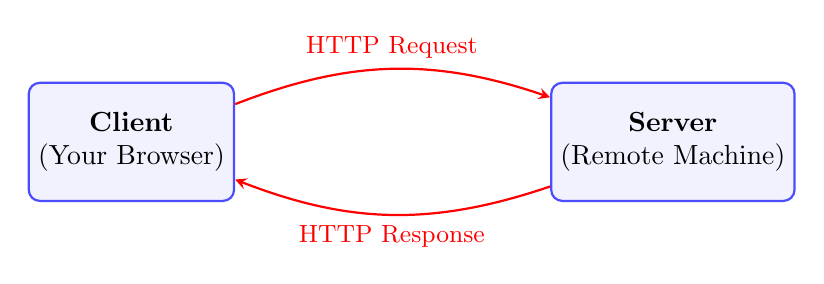
\begin{tikzpicture}[
    node distance=3cm,
    box/.style={rectangle, rounded corners, draw=blue!70, fill=blue!5, thick, minimum width=2.5cm, minimum height=1.5cm, align=center},
    arrow/.style={->, >=stealth, thick, red}
]

\node[box] (client) {\textbf{Client}\\(Your Browser)};
\node[box, right=4cm of client] (server) {\textbf{Server}\\(Remote Machine)};

\draw[arrow, bend left=20] (client) to node[above, font=\small] {HTTP Request} (server);
\draw[arrow, bend left=20] (server) to node[below, font=\small] {HTTP Response} (client);

\end{tikzpicture}
\end{center}

\begin{itemize}[leftmargin=*]
    \item \textbf{Client}: Requests something from server
    \item \textbf{Server}: Responds to client's request
    \item \textbf{Protocol}: Communication happens via HTTP (Hypertext Transfer Protocol)
\end{itemize}

\subsection{Website Classification}

Just like software, websites are also classified:

\subsubsection{Static Websites}

\begin{itemize}[leftmargin=*]
    \item Minimal user interaction
    \item Primarily for displaying information
    \item Examples: Blogs, government websites
    \item One-way information flow
\end{itemize}

\subsubsection{Dynamic Websites}

\begin{itemize}[leftmargin=*]
    \item High user interaction
    \item Active data manipulation
    \item Examples: Instagram, Facebook, Zomato
    \item Two-way communication
\end{itemize}

\subsection{CRUD in Dynamic Websites}

\begin{notebox}
\textbf{Key Point}: The same CRUD principle applies to websites! No matter how many interactions a website allows, they all fall into these four categories.
\end{notebox}

\subsubsection{Instagram Example}

Let's analyze Instagram interactions:

\vspace{0.5em}

\textbf{Create Operations}:
\begin{itemize}[leftmargin=*]
    \item Upload new photo/video posts
    \item Write new comments
    \item Create stories
    \item Send new messages
\end{itemize}

\textbf{Retrieve Operations}:
\begin{itemize}[leftmargin=*]
    \item Scroll through feed
    \item View someone's profile
    \item Read comments
    \item View stories
\end{itemize}

\textbf{Update Operations}:
\begin{itemize}[leftmargin=*]
    \item Edit your profile
    \item Edit your comments
    \item Update bio
\end{itemize}

\textbf{Delete Operations}:
\begin{itemize}[leftmargin=*]
    \item Delete your posts
    \item Delete your comments
    \item Remove followers
\end{itemize}

\subsubsection{Zomato Example}


\textbf{Create}: Place a new order
\vspace{0.3em}
\textbf{Retrieve}: View past orders
\vspace{0.3em}
\textbf{Update}: Update delivery address
\vspace{0.3em}
\textbf{Delete}: Delete saved address

\newpage

% ========================
% SECTION 3: HTTP METHODS DEEP DIVE
% ========================
\section{HTTP Methods (Verbs)}

\subsection{The Communication Challenge}

Since dynamic websites communicate over the internet (client $\leftrightarrow$ server via HTTP), there's an important requirement:

\begin{warningbox}
\textbf{Critical Requirement}: When performing any CRUD operation, the HTTP request MUST specify which type of interaction you want to perform!
\end{warningbox}

\textbf{Why?}
\begin{itemize}[leftmargin=*]
    \item HTTP requests travel over the internet
    \item Server needs to understand what the client wants
    \item Different operations require different handling
    \item Ambiguity would cause errors
\end{itemize}

\subsection{HTTP Verbs/Methods}

To specify the type of interaction, we add a \textbf{verb} to the HTTP request. These verbs are called \textbf{HTTP Methods}.

\begin{center}
\begin{tabular}{|l|l|p{0.5\textwidth}|}
\hline
\textbf{CRUD} & \textbf{HTTP Method} & \textbf{Purpose} \\
\hline
\textbf{Create} & \textbf{POST} & Send data to server to create new resource \\
\hline
\textbf{Retrieve} & \textbf{GET} & Request data from server \\
\hline
\textbf{Update} & \textbf{PUT/PATCH} & Modify existing resource on server \\
\hline
\textbf{Delete} & \textbf{DELETE} & Remove resource from server \\
\hline
\end{tabular}
\end{center}

\subsection{The GET Method}

\textbf{Purpose}: Retrieve/Read data from server

\vspace{0.5em}
\textbf{When to use}:
\begin{itemize}[leftmargin=*]
    \item Viewing a profile page
    \item Scrolling through feed
    \item Reading comments
    \item Accessing any page
\end{itemize}

\begin{examplebox}{GET Request Example}
\textbf{Scenario}: You want to view your profile page on a website

\vspace{0.5em}
\textbf{What happens}:
\begin{enumerate}[leftmargin=*]
    \item Your browser sends HTTP request with GET method
    \item Request includes: "I want to retrieve my profile page"
    \item Server understands this is a retrieve operation
    \item Server sends back the profile page data
\end{enumerate}

\textbf{Request format}:
\begin{verbatim}
GET /profile HTTP/1.1
Host: example.com
\end{verbatim}
\end{examplebox}

\subsection{The POST Method}

\textbf{Purpose}: Send data to server to create new resources

\vspace{0.5em}
\textbf{When to use}:
\begin{itemize}[leftmargin=*]
    \item Submitting login form
    \item Submitting registration form
    \item Uploading a new post
    \item Sending any form data
\end{itemize}

\begin{examplebox}{POST Request Example}
\textbf{Scenario}: You're filling a login form

\vspace{0.5em}
\textbf{What happens}:
\begin{enumerate}[leftmargin=*]
    \item You enter email and password
    \item Click "Login" button
    \item Browser sends HTTP request with POST method
    \item Request body contains your credentials
    \item Server receives and processes the data
\end{enumerate}

\textbf{Request format}:
\begin{verbatim}
POST /authenticate HTTP/1.1
Host: example.com
Content-Type: application/json

{
    "email": "user@example.com",
    "password": "password123"
}
\end{verbatim}
\end{examplebox}

\subsection{The PUT Method}

\textbf{Purpose}: Update/Modify existing resource

\vspace{0.5em}
\textbf{When to use}:
\begin{itemize}[leftmargin=*]
    \item Editing profile information
    \item Updating a post
    \item Modifying settings
    \item Changing existing data
\end{itemize}

\begin{examplebox}{PUT Request Example}
\textbf{Scenario}: Updating your profile bio

\vspace{0.5em}
\textbf{What happens}:
\begin{enumerate}[leftmargin=*]
    \item You edit your bio
    \item Click "Save"
    \item Browser sends HTTP request with PUT method
    \item Server updates your profile
\end{enumerate}
\end{examplebox}

\subsection{The DELETE Method}

\textbf{Purpose}: Remove resource from server

\vspace{0.5em}
\textbf{When to use}:
\begin{itemize}[leftmargin=*]
    \item Deleting a post
    \item Removing a comment
    \item Deleting an account
    \item Removing any data
\end{itemize}

\subsection{HTTP Methods Summary}

\begin{infobox}{Key Concept}
For EVERY type of interaction in the HTTP body, you send a verb. These verbs collectively are called \textbf{HTTP Methods}.
\end{infobox}

\textbf{Most commonly used}:
\begin{itemize}[leftmargin=*]
    \item \textbf{GET and POST}: Used most frequently
    \item \textbf{PUT and DELETE}: Used less frequently but still important
\end{itemize}

\begin{notebox}
These four HTTP methods are essential knowledge for anyone building websites or APIs. They form the foundation of REST API design.
\end{notebox}

\newpage

% ========================
% SECTION 4: LIVE DEMONSTRATION
% ========================
\section{HTTP Methods in Action}

Let's see HTTP methods in real-world usage by inspecting browser network traffic.

\subsection{Inspecting Network Requests}

\subsubsection{Setup}

To view HTTP methods in your browser:

\begin{enumerate}[leftmargin=*]
    \item Open any website
    \item Right-click and select "Inspect" (or press F12)
    \item Go to the "Network" tab
    \item Perform actions on the website
    \item Watch requests appear in the network tab
\end{enumerate}

\subsection{Example 1: GET Request}

\subsubsection{Scenario: Accessing a Courses Page}

\hspace{1.5em}\textbf{Action}: Click on "Courses" link

\vspace{0.5em}
\textbf{Operation Type}: Retrieve/Read (viewing a page)

\vspace{0.5em}
\textbf{Expected Method}: GET

\begin{examplebox}{Network Tab Observation}
\begin{verbatim}
Request URL: https://example.com/store
Request Method: GET
Status Code: 200 OK
\end{verbatim}

\textbf{What we see}:
\begin{itemize}[leftmargin=*]
    \item Request URL shows the page we're accessing
    \item Request Method is GET (as expected)
    \item This confirms: viewing a page uses GET
\end{itemize}
\end{examplebox}

\subsection{Example 2: POST Request}

\subsubsection{Scenario: Logging In}

\hspace{1.5em}\textbf{Action}: Fill login form and click "Login"

\vspace{0.5em}
\textbf{Operation Type}: Create (sending data to server)

\vspace{0.5em}
\textbf{Expected Method}: POST

\begin{examplebox}{Login Form Submission}
\textbf{Steps}:
\begin{enumerate}[leftmargin=*]
    \item Click "Login" button
    \item Click "Continue with Email"
    \item Enter email: dummy@gmail.com
    \item Enter password: 1234 (intentionally wrong)
    \item Click "Next"
\end{enumerate}

\textbf{Network Tab Observation}:
\begin{verbatim}
Request URL: https://example.com/authenticate
Request Method: POST
Status Code: 401 Unauthorized
\end{verbatim}

\textbf{What we see}:
\begin{itemize}[leftmargin=*]
    \item Request URL: /authenticate endpoint
    \item Request Method: POST (as expected)
    \item This confirms: sending form data uses POST
    \item Status 401: Authentication failed (wrong password)
\end{itemize}
\end{examplebox}

\subsection{Key Observations}

\begin{infobox}{Understanding HTTP Methods in Practice}
\textbf{GET Requests}:
\begin{itemize}[leftmargin=*]
    \item Triggered when viewing pages
    \item No data sent in body
    \item Just retrieving information
\end{itemize}

\textbf{POST Requests}:
\begin{itemize}[leftmargin=*]
    \item Triggered when submitting forms
    \item Data sent in request body
    \item Creating or sending information
\end{itemize}
\end{infobox}

\newpage

% ========================
% SECTION 5: PROJECT SETUP
% ========================
\section{Starting the Project}

Now that we understand HTTP methods, let's start building our Patient Management API!

\subsection{Environment Setup}

\subsubsection{Activating Virtual Environment}

\begin{cmdbox}
\begin{verbatim}
# Windows
env\Scripts\activate.bat

# Linux/Mac
source env/bin/activate
\end{verbatim}
\end{cmdbox}

\subsection{Creating the Data File}

\subsubsection{patients.json Structure}

Create a file named \texttt{patients.json} with sample data:

\begin{lstlisting}[language=Python]
{
  "P001": {
    "name": "Ananya Verma",
    "city": "Guwahati",
    "age": 28,
    "gender": "female",
    "height": 1.65,
    "weight": 90.0,
    "bmi": 33.06,
    "verdict": "Obese"
  },
  "P002": {
    "name": "Ravi Mehta",
    "city": "Mumbai",
    "age": 35,
    "gender": "male",
    "height": 1.75,
    "weight": 85,
    "bmi": 27.76,
    "verdict": "Overweight"
  },
  "P003": {
    "name": "Sneha Kulkarni",
    "city": "Pune",
    "age": 22,
    "gender": "female",
    "height": 1.6,
    "weight": 45,
    "bmi": 17.58,
    "verdict": "Underweight"
  },
  "P004": {
    "name": "Arjun Verma",
    "city": "Mumbai",
    "age": 40,
    "gender": "male",
    "height": 1.8,
    "weight": 90.0,
    "bmi": 27.78,
    "verdict": "Normal"
  },
  "P005": {
    "name": "Neha Sinha",
    "city": "Kolkata",
    "age": 30,
    "gender": "female",
    "height": 1.55,
    "weight": 75,
    "bmi": 31.22,
    "verdict": "Obese"
  }
}
\end{lstlisting}

\begin{notebox}
This JSON file acts as our "database" for this learning project. Each patient has a unique ID (P001, P002, etc.) and stores all relevant information. As new patients are added, they'll be appended to this file.
\end{notebox}

\subsection{Understanding the Data Structure}

Each patient record contains:
\begin{itemize}[leftmargin=*]
    \item \textbf{Patient ID}: Unique identifier (P001, P002, etc.)
    \item \textbf{name}: Patient's full name
    \item \textbf{city}: Location
    \item \textbf{age}: Patient's age in years
    \item \textbf{gender}: Male/Female
    \item \textbf{height}: Height in meters
    \item \textbf{weight}: Weight in kilograms
    \item \textbf{bmi}: Body Mass Index (calculated)
    \item \textbf{verdict}: Health status based on BMI
\end{itemize}

\newpage

% ========================
% SECTION 6: BUILDING THE API
% ========================
\section{Building the First API Endpoint}

\subsection{Modifying Existing Code}

Let's update our basic FastAPI app from the previous session.

\subsubsection{Updated main.py - Initial Version}

\begin{lstlisting}[language=Python]
from fastapi import FastAPI

app = FastAPI()

@app.get("/")
def hello():
    return {"message": "Hello World"}

@app.get("/about")
def about():
    return {"message": "This is the about page"}
\end{lstlisting}

\subsubsection{Updated main.py - Modified Version}

\begin{lstlisting}[language=Python]
from fastapi import FastAPI

app = FastAPI()

@app.get("/")
def hello():
    return {"message": "Patient Management System API"}

@app.get("/about")
def about():
    return {"message": "A fully functional API to manage patient records"}
\end{lstlisting}

\subsection{Creating a Helper Function}

Before building endpoints, we need a reusable function to load data from the JSON file.

\subsubsection{Why We Need a Helper Function}

\begin{itemize}[leftmargin=*]
    \item We'll need to read from patients.json repeatedly
    \item Multiple endpoints will require patient data
    \item Better to write once and reuse
    \item Follows DRY principle (Don't Repeat Yourself)
\end{itemize}

\subsubsection{The load\_data() Function}

\begin{lstlisting}[language=Python]
import json

def load_data():
    """
    Helper function to load patient data from JSON file
    Returns: Dictionary containing all patient records
    """
    with open("patients.json", "r") as f:
        data = json.load(f)
    
    return data
\end{lstlisting}

\textbf{How it works}:
\begin{enumerate}[leftmargin=*]
    \item Opens the patients.json file in read mode
    \item Uses json.load() to parse the JSON data
    \item Returns the data as a Python dictionary
    \item Can be called anytime we need patient data
\end{enumerate}

\subsection{Building the View All Patients Endpoint}

\subsubsection{Endpoint Specification}

\begin{infobox}{Endpoint Details}
\textbf{Route}: /view

\textbf{HTTP Method}: GET (retrieving data)

\textbf{Purpose}: Return all patient records

\textbf{Response}: Complete JSON data from patients.json
\end{infobox}

\subsubsection{Complete Code}

\begin{lstlisting}[language=Python]
from fastapi import FastAPI
import json

app = FastAPI()

def load_data():
    """Load patient data from JSON file"""
    with open("patients.json", "r") as f:
        data = json.load(f)
    return data

@app.get("/")
def hello():
    return {"message": "Patient Management System API"}

@app.get("/about")
def about():
    return {"message": "A fully functional API to manage patient records"}

@app.get("/view")
def view():
    """
    Endpoint to retrieve all patient records
    Returns: All patient data from JSON file
    """
    data = load_data()
    return data
\end{lstlisting}

\subsection{Code Explanation}

\subsubsection{Import Statements}

\begin{lstlisting}[language=Python]
from fastapi import FastAPI
import json
\end{lstlisting}

\begin{itemize}[leftmargin=*]
    \item \texttt{FastAPI}: Core framework for building the API
    \item \texttt{json}: Module for parsing JSON files
\end{itemize}

\subsubsection{The View Endpoint}

\begin{lstlisting}[language=Python]
@app.get("/view")
def view():
    data = load_data()
    return data
\end{lstlisting}

\textbf{Step-by-step execution}:
\begin{enumerate}[leftmargin=*]
    \item Decorator \texttt{@app.get("/view")} defines route and method
    \item Function \texttt{view()} handles requests to this endpoint
    \item Calls \texttt{load\_data()} to fetch all patient records
    \item Returns data as JSON response automatically
\end{enumerate}

\begin{notebox}
FastAPI automatically converts Python dictionaries to JSON format in the HTTP response. You don't need to manually serialize the data!
\end{notebox}

\newpage

% ========================
% SECTION 7: RUNNING THE API
% ========================
\section{Testing the API}

\subsection{Starting the Server}

\subsubsection{Using Uvicorn}

\begin{cmdbox}
\begin{verbatim}
uvicorn main:app --reload
\end{verbatim}
\end{cmdbox}

\textbf{Command breakdown}:
\begin{itemize}[leftmargin=*]
    \item \texttt{uvicorn}: ASGI server for running FastAPI
    \item \texttt{main}: Name of Python file (main.py)
    \item \texttt{app}: Name of FastAPI instance
    \item \texttt{--reload}: Auto-reload on code changes (development only)
\end{itemize}

\subsubsection{Server Output}

\begin{verbatim}
INFO:     Uvicorn running on http://127.0.0.1:8000
INFO:     Application startup complete.
\end{verbatim}

Your API is now running at: \texttt{http://127.0.0.1:8000}

\subsection{Testing Endpoints in Browser}

\subsubsection{Home Endpoint}

\hspace{1.5em}\textbf{URL}: \texttt{http://127.0.0.1:8000/}

\vspace{0.5em}
\textbf{Response}:
\begin{verbatim}
{
    "message": "Patient Management System API"
}
\end{verbatim}

\subsubsection{About Endpoint}

\hspace{1.5em}\textbf{URL}: \texttt{http://127.0.0.1:8000/about}

\vspace{0.5em}
\textbf{Response}:
\begin{verbatim}
{
    "message": "A fully functional API to manage patient records"
}
\end{verbatim}

\subsubsection{View All Patients Endpoint}

\hspace{1.5em}\textbf{URL}: \texttt{http://127.0.0.1:8000/view}

\vspace{0.5em}
\textbf{Response}: (Complete patient data)
\begin{lstlisting}[language=Python]
{
  "P001": {
    "name": "Ananya Verma",
    "city": "Guwahati",
    "age": 28,
    "gender": "female",
    "height": 1.65,
    "weight": 90.0,
    "bmi": 33.06,
    "verdict": "Obese"
  },
  "P002": {
    "name": "Ravi Mehta",
    "city": "Mumbai",
    "age": 35,
    "gender": "male",
    "height": 1.75,
    "weight": 85,
    "bmi": 27.76,
    "verdict": "Overweight"
  },
  // ... rest of the patient data
}
\end{lstlisting}

\subsection{Using FastAPI's Interactive Documentation}

\subsubsection{Accessing Swagger UI}

FastAPI automatically generates interactive API documentation!

\vspace{0.5em}
\textbf{URL}: \texttt{http://127.0.0.1:8000/docs}

\begin{infobox}{Automatic Documentation}
FastAPI uses OpenAPI standards to create beautiful, interactive documentation. This is one of FastAPI's killer features - you get professional API docs without writing a single line of documentation code!
\end{infobox}

\subsubsection{Testing in Swagger UI}

\begin{enumerate}[leftmargin=*]
    \item Navigate to \texttt{http://127.0.0.1:8000/docs}
    \item You'll see all available endpoints listed
    \item Find the \texttt{GET /view} endpoint
    \item Click to expand it
    \item Click "Try it out" button
    \item Click "Execute" button
    \item View the response below
\end{enumerate}

\begin{examplebox}{Swagger UI Response}
\textbf{Response Code}: 200 OK

\textbf{Response Body}: Shows all patient data

\textbf{Response Headers}: Content-Type: application/json

\vspace{0.5em}
This confirms our endpoint is working perfectly!
\end{examplebox}

\subsection{Understanding the Response}

\subsubsection{What Happens When You Access /view}

\begin{center}
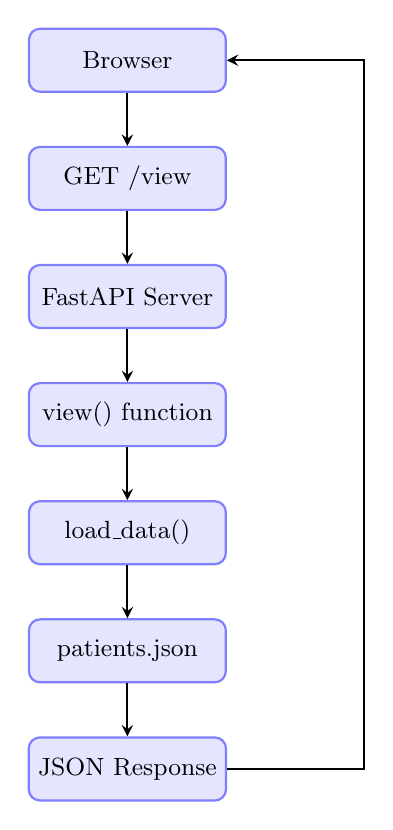
\begin{tikzpicture}[
    node distance=1.5cm,
    process/.style={rectangle, rounded corners, draw=blue!50, fill=blue!10, thick, minimum width=2.5cm, minimum height=0.8cm, font=\small},
    arrow/.style={->, >=stealth, thick}
]

\node[process] (browser) {Browser};
\node[process, below of=browser] (request) {GET /view};
\node[process, below of=request] (fastapi) {FastAPI Server};
\node[process, below of=fastapi] (function) {view() function};
\node[process, below of=function] (helper) {load\_data()};
\node[process, below of=helper] (json) {patients.json};
\node[process, below of=json] (response) {JSON Response};

\draw[arrow] (browser) -- (request);
\draw[arrow] (request) -- (fastapi);
\draw[arrow] (fastapi) -- (function);
\draw[arrow] (function) -- (helper);
\draw[arrow] (helper) -- (json);
\draw[arrow] (json) -- (response);
\draw[arrow] (response) -- ++(3,0) |- (browser);

\end{tikzpicture}
\end{center}

\textbf{Step-by-step flow}:
\begin{enumerate}[leftmargin=*]
    \item Browser sends GET request to /view
    \item FastAPI routes request to view() function
    \item view() calls load\_data() helper function
    \item load\_data() opens and reads patients.json
    \item Data returned to view() function
    \item view() returns data to FastAPI
    \item FastAPI serializes to JSON and sends response
    \item Browser receives and displays the data
\end{enumerate}

\newpage

% ========================
% SECTION 8: COMPLETE CODE OVERVIEW
% ========================
\section{Complete Code Reference}

\subsection{Final main.py}

\begin{lstlisting}[language=Python]
from fastapi import FastAPI
import json

app = FastAPI()

def load_data():
    """
    Helper function to load patient data from JSON file.
    
    Returns:
        dict: Dictionary containing all patient records
    """
    with open("patients.json", "r") as f:
        data = json.load(f)
    return data

@app.get("/")
def hello():
    """
    Home endpoint - API welcome message.
    
    Returns:
        dict: Welcome message
    """
    return {"message": "Patient Management System API"}

@app.get("/about")
def about():
    """
    About endpoint - API description.
    
    Returns:
        dict: API description message
    """
    return {"message": "A fully functional API to manage patient records"}

@app.get("/view")
def view():
    """
    View all patients endpoint.
    Retrieves and returns all patient records from the database.
    
    Returns:
        dict: Complete patient data with all records
    """
    data = load_data()
    return data
\end{lstlisting}

\newpage

\subsection{patients.json Structure}

\begin{lstlisting}[language=Python]
{
  "P001": {
    "name": "Ananya Verma",
    "city": "Guwahati",
    "age": 28,
    "gender": "female",
    "height": 1.65,
    "weight": 90.0,
    "bmi": 33.06,
    "verdict": "Obese"
  },
  "P002": {
    "name": "Ravi Mehta",
    "city": "Mumbai",
    "age": 35,
    "gender": "male",
    "height": 1.75,
    "weight": 85,
    "bmi": 27.76,
    "verdict": "Overweight"
  },
  "P003": {
    "name": "Sneha Kulkarni",
    "city": "Pune",
    "age": 22,
    "gender": "female",
    "height": 1.6,
    "weight": 45,
    "bmi": 17.58,
    "verdict": "Underweight"
  },
  "P004": {
    "name": "Arjun Verma",
    "city": "Mumbai",
    "age": 40,
    "gender": "male",
    "height": 1.8,
    "weight": 90.0,
    "bmi": 27.78,
    "verdict": "Normal"
  },
  "P005": {
    "name": "Neha Sinha",
    "city": "Kolkata",
    "age": 30,
    "gender": "female",
    "height": 1.55,
    "weight": 75,
    "bmi": 31.22,
    "verdict": "Obese"
  }
}
\end{lstlisting}

\subsection{Project Structure}

\begin{cmdbox}
\begin{verbatim}
patient-management-api/
|-- env/                    # Virtual environment
|-- main.py                 # FastAPI application
|-- patients.json           # Patient database (JSON)
|-- requirements.txt        # Python dependencies
\end{verbatim}
\end{cmdbox}

\subsection{requirements.txt}

\begin{lstlisting}[language=bash]
fastapi==0.104.1
uvicorn[standard]==0.24.0
pydantic==2.5.0
\end{lstlisting}

\newpage


% ========================
% SECTION 10: KEY CONCEPTS SUMMARY
% ========================
\section{Key Concepts Summary}

\subsection{What We Learned}

\subsubsection{1. Project Understanding}

\begin{itemize}[leftmargin=*]
    \item Real-world problem: Digitizing patient records
    \item Solution: REST API for patient management
    \item Backend focus: We build the API, not the app
    \item Storage: JSON file (learning project) vs Database (production)
\end{itemize}

\subsubsection{2. Software Classification}

\begin{center}
\begin{tabular}{|l|l|}
\hline
\textbf{Static Software} & \textbf{Dynamic Software} \\
\hline
Minimal interaction & High interaction \\
One-way communication & Two-way communication \\
Examples: Calendar, Clock & Examples: Excel, Instagram \\
\hline
\end{tabular}
\end{center}

\subsubsection{3. CRUD Operations}

\begin{infobox}{Universal Pattern}
ALL dynamic software/websites support only 4 types of interactions:

\begin{itemize}[leftmargin=*]
    \item \textbf{C}reate: Adding new data
    \item \textbf{R}etrieve: Reading existing data
    \item \textbf{U}pdate: Modifying existing data
    \item \textbf{D}elete: Removing data
\end{itemize}
\end{infobox}

\subsubsection{4. HTTP Methods}

\begin{center}
\begin{tabular}{|l|l|l|}
\hline
\textbf{CRUD} & \textbf{HTTP Method} & \textbf{Usage} \\
\hline
Create & POST & Submit forms, create resources \\
\hline
Retrieve & GET & View pages, fetch data \\
\hline
Update & PUT/PATCH & Modify existing resources \\
\hline
Delete & DELETE & Remove resources \\
\hline
\end{tabular}
\end{center}

\subsubsection{5. Client-Server Architecture}

\begin{itemize}[leftmargin=*]
    \item \textbf{Client}: User's browser/device (sends requests)
    \item \textbf{Server}: Remote machine hosting the API (sends responses)
    \item \textbf{Protocol}: HTTP (communication standard)
    \item \textbf{Request}: Contains method, URL, headers, body
    \item \textbf{Response}: Contains status code, headers, body
\end{itemize}

\subsubsection{6. FastAPI Basics}

\begin{itemize}[leftmargin=*]
    \item Framework for building APIs in Python
    \item Automatic JSON serialization
    \item Built-in interactive documentation
    \item Type hints and data validation
    \item Fast performance (async support)
\end{itemize}

\subsection{Practical Implementation}

\subsubsection{What We Built}

\begin{enumerate}[leftmargin=*]
    \item \textbf{Home Endpoint} (/): Welcome message
    \item \textbf{About Endpoint} (/about): API description
    \item \textbf{View All Endpoint} (/view): Get all patient records
\end{enumerate}

\subsubsection{Code Structure}

\begin{lstlisting}[language=Python]
# 1. Import necessary modules
from fastapi import FastAPI
import json

# 2. Create FastAPI instance
app = FastAPI()

# 3. Helper function
def load_data():
    # Load data from JSON file
    pass

# 4. Define endpoints
@app.get("/route")
def function_name():
    # Endpoint logic
    return response_data
\end{lstlisting}

\subsection{Important Principles}

\begin{infobox}{Best Practices}
\begin{enumerate}[leftmargin=*]
    \item \textbf{DRY Principle}: Don't Repeat Yourself (use helper functions)
    \item \textbf{RESTful Design}: Follow REST conventions for API design
    \item \textbf{Clear Naming}: Use descriptive function and variable names
    \item \textbf{Proper HTTP Methods}: Use correct method for each operation
    \item \textbf{Documentation}: Write docstrings for functions
    \item \textbf{Error Handling}: Plan for failure cases
    \item \textbf{Consistent Response Format}: Standardize API responses
\end{enumerate}
\end{infobox}

\newpage

% ========================
% SECTION 11: TROUBLESHOOTING
% ========================
\section{Common Issues and Solutions}

\subsection{Server Won't Start}

\subsubsection{Problem: ModuleNotFoundError}

\begin{verbatim}
ModuleNotFoundError: No module named 'fastapi'
\end{verbatim}

\textbf{Solution}:
\begin{cmdbox}
\begin{verbatim}
# Ensure virtual environment is activated
# Then install FastAPI
pip install fastapi uvicorn
\end{verbatim}
\end{cmdbox}

\subsubsection{Problem: Port Already in Use}

\begin{verbatim}
ERROR: [Errno 48] Address already in use
\end{verbatim}

\textbf{Solution}:
\begin{cmdbox}
\begin{verbatim}
# Use different port
uvicorn main:app --reload --port 8001

# Or kill existing process on port 8000
# Windows:
netstat -ano | findstr :8000
taskkill /PID <PID> /F

# Linux/Mac:
lsof -ti:8000 | xargs kill
\end{verbatim}
\end{cmdbox}

\subsection{JSON File Issues}

\subsubsection{Problem: FileNotFoundError}

\begin{verbatim}
FileNotFoundError: [Errno 2] No such file or directory: 'patients.json'
\end{verbatim}

\textbf{Solution}:
\begin{itemize}[leftmargin=*]
    \item Ensure patients.json is in the same directory as main.py
    \item Check file name spelling (case-sensitive)
    \item Verify file path in load\_data() function
\end{itemize}

\subsubsection{Problem: JSON Decode Error}

\begin{verbatim}
json.decoder.JSONDecodeError: Expecting property name enclosed in double quotes
\end{verbatim}

\textbf{Solution}:
\begin{itemize}[leftmargin=*]
    \item Validate JSON syntax at jsonlint.com
    \item Ensure all keys are in double quotes
    \item Check for trailing commas
    \item Verify proper bracket/brace closure
\end{itemize}

\subsection{Browser Issues}

\subsubsection{Problem: 404 Not Found}

\textbf{Causes and Solutions}:
\begin{itemize}[leftmargin=*]
    \item Wrong URL: Check spelling of endpoint
    \item Server not running: Ensure uvicorn is active
    \item Wrong port: Verify you're using correct port number
\end{itemize}

\subsubsection{Problem: Empty Response}

\textbf{Solutions}:
\begin{itemize}[leftmargin=*]
    \item Check if patients.json has data
    \item Verify load\_data() returns data correctly
    \item Check browser console for errors
\end{itemize}

\newpage

% ========================
% SECTION 13: QUICK REFERENCE
% ========================
\section{Quick Reference Guide}

\subsection{Essential Commands}

\begin{tcolorbox}[colback=blue!5!white,colframe=blue!75!black,title=Virtual Environment]
\begin{verbatim}
# Create virtual environment
python -m venv env

# Activate (Windows)
env\Scripts\activate.bat

# Activate (Linux/Mac)
source env/bin/activate

# Deactivate
deactivate
\end{verbatim}
\end{tcolorbox}

\begin{tcolorbox}[colback=green!5!white,colframe=green!75!black,title=Installation]
\begin{verbatim}
# Install FastAPI and Uvicorn
pip install fastapi uvicorn[standard]

# Install from requirements.txt
pip install -r requirements.txt

# Create requirements.txt
pip freeze > requirements.txt
\end{verbatim}
\end{tcolorbox}

\begin{tcolorbox}[colback=orange!5!white,colframe=orange!75!black,title=Running Server]
\begin{verbatim}
# Basic command
uvicorn main:app

# With auto-reload (development)
uvicorn main:app --reload

# Custom port
uvicorn main:app --reload --port 8001

# Custom host (accessible from network)
uvicorn main:app --host 0.0.0.0 --port 8000
\end{verbatim}
\end{tcolorbox}

\subsection{FastAPI Endpoint Template}

\begin{lstlisting}[language=Python]
from fastapi import FastAPI

app = FastAPI()

@app.get("/endpoint")           # HTTP Method and Route
def function_name():            # Function name
    """
    Endpoint description
    """
    # Your logic here
    return {"key": "value"}     # Return dictionary (becomes JSON)
\end{lstlisting}

\subsection{HTTP Methods Reference}

\begin{center}
\begin{tabular}{|l|l|p{0.5\textwidth}|}
\hline
\textbf{Method} & \textbf{Decorator} & \textbf{Purpose} \\
\hline
GET & @app.get() & Retrieve data, read operations \\
\hline
POST & @app.post() & Create new resources, submit data \\
\hline
PUT & @app.put() & Update entire resource \\
\hline
PATCH & @app.patch() & Partial update of resource \\
\hline
DELETE & @app.delete() & Delete resource \\
\hline
\end{tabular}
\end{center}

\subsection{Common HTTP Status Codes}

\begin{center}
\begin{tabular}{|l|l|p{0.5\textwidth}|}
\hline
\textbf{Code} & \textbf{Status} & \textbf{Meaning} \\
\hline
200 & OK & Request succeeded \\
\hline
201 & Created & Resource created successfully \\
\hline
400 & Bad Request & Invalid request data \\
\hline
401 & Unauthorized & Authentication required \\
\hline
404 & Not Found & Resource not found \\
\hline
500 & Internal Server Error & Server error \\
\hline
\end{tabular}
\end{center}

\vfill

\begin{center}
\textit{End of FastAPI Patient Management System Guide - Session 1}

\vspace{1em}

\textit{"The only way to learn a new programming language is by writing programs in it."}\\
\textit{— Dennis Ritchie}

\vspace{1em}

\textbf{Keep coding, keep learning!}\\
See you in the next session where we'll implement more CRUD operations!
\end{center}

\end{document}